\section{Optimal Control of Pitch/Travel and Elevation with and without Feedback}\label{sec:prob4}
\label{text:problem4}

Refer to system id TF for elevation, and we get the following extended continuous state space model:

\subsection{State space model}
We wish to calculate an optimal trajectory in two dimension, adding a constraint to the elevation. Adding $e$ and $\dot{e}$ to the previous state space model \eqref{eq:sys}, we get
\begin{equation}
	\begin{bmatrix}
		\dot{\lambda}\\
		\ddot{\lambda}	\\
		\dot{p}	\\
		\ddot{p}\\
		\dot{e}	\\
		\ddot{e}
	\end{bmatrix} = 
	\underbrace{
	\begin{bmatrix}
		0 & 1 & 0 & 0 & 0  & 0 \\
		0 & -0.03 & -0.39 & 0 & 0 & 0 \\
		0 & 0 & 0 & 1 & 0 & 0 \\
		0 & 0 & -7.13 & -3.6 & 0 & 0 \\
		0 & 0 & 0 & 0 & 0 & 1 \\
		0 & 0 & 0 & 1 & -3.03 & -2.44 \\
	\end{bmatrix}}_{A_c}
	\begin{bmatrix}
		\lambda	\\
		\dot{\lambda}\\
		p		\\
		\dot{p} \\
		e		\\
		\dot{e}
	\end{bmatrix} +
	\underbrace{
	\begin{bmatrix}
		0 & 0\\
		0 & 0\\
		0 & 0\\
		6.74 & 0\\
		0 & 0 \\
		0 & 3.13 \\
	\end{bmatrix}}_{B_c}
	\begin{bmatrix}
	p_c \\
	e_c
	\end{bmatrix}
	\label{eq:ex_sys}
\end{equation}

Discuss decoupling...?

\subsection{Discretization}
Now let $x = \begin{bmatrix}\lambda&\dot{\lambda}&p&\dot{p}&e&\dot{e}\end{bmatrix}^\top$, $u = \begin{bmatrix}p_c&e_c\end{bmatrix}^\top$. Again, using approximate discretization via Euler we obtain a discrete state space model
\begin{subequations}
\begin{align}
	\label{eq:ex_dsys}
	x_{k+1} &= (I + \Delta t A_c) x_k + (\Delta t B_c) u_k. \\
	&= Ax_k + Bu_k,
\end{align}
\end{subequations}

where 
\begin{equation*}
	A = 
	\begin{bmatrix}
		1 & 0.25 & 0 & 0 & 0 & 0\\
		0 & 0.9925 & -0.0975 & 0 & 0 & 0\\
		0 & 0 & 1 & 0.25 & 0 & 0\\
		0 & 0 & -1.7825 & 0.1 & 0 & 0\\
		0 & 0 & 0 & 0 & 1 & 0.25\\
		0 & 0 & 0 & 0 & -0.7575 & 0.39
	\end{bmatrix}, \quad
	B = 
	\begin{bmatrix}
		0 & 0\\
		0 & 0\\
		0 & 0\\
		1.685 & 0\\
		0 & 0\\
		0 & 0.7825
	\end{bmatrix}.
\end{equation*}

\subsection{Optimization problem with nonlinear constraints}

We calculate an optimal trajectory from $x_0 = \begin{bmatrix}\lambda_0&0&0&0&0&0\end{bmatrix}^\top$ to $x_f = \begin{bmatrix}\lambda_f&0&0&0&0&0\end{bmatrix}^\top$ minimizing the objective function 
\begin{equation*}
	\phi = \sum_{i=1}^{N}(\lambda_i - \lambda_f)^2 + r_1 p^2_{c_i} + r_2 e^2_{c_i}, \quad r_1,r_2 \ge 0,
\end{equation*}

or alternatively
\begin{equation}
	\label{eq:quad_cost}
	\phi = \sum_{i=0}^{N-1} (x_{i+1}-x_f)^\top Q(x_{i+1}-x_f) + u_i^\top R u_i,
\end{equation}
where

\begin{equation}
Q = \begin{bmatrix}1&0&0&0&0&0\\0&0&0&0&0&0\\0&0&0&0&0&0\\0&0&0&0&0&0\\0&0&0&0&0&0\\0&0&0&0&0&0\end{bmatrix}, \quad R = \begin{bmatrix}r_1&0\\0&r_2\end{bmatrix}.
\end{equation}

 The second weighting parameter $r_2$ is added as we impose an inequality constraint on the elevation for every time step:

\begin{equation}
	\label{eq:cons}
	c(x_k) = \alpha \exp{\left(-\beta\left(\lambda_k - \lambda_t\right)^2\right)} - e_k \le 0, \quad k = \{1, \dots , N\},
\end{equation}
where we let $\alpha = 0.2$, $\beta = 20$, $\lambda_t = \frac{2\pi}{3}$.

The objective function \eqref{eq:quad_cost} is subject to the system dynamics \eqref{eq:ex_dsys} and thus imposed to linear equality constraints identically defined to that of \eqref{eq:eq_constraints}. Similarly to \eqref{eq:QP_travel} we define the optimization variable $z$ and the matrix $G$, and the resulting optimization problem can be stated:
\begin{subequations}
\label{eq:NOP}
	\begin{equation}
		\min_z \quad z^T G z
	\end{equation}
subject to
\begin{align}
	A_{eq} z &= B_{eq}, \\
	c(x_k) &\le 0, \quad k = \{1, \dots N\},\\
	p^{\textrm{low}} \le p_k &\le p^{\textrm{high}}, \quad k = \{1, \dots N\}.
\end{align}
\end{subequations}


\subsection{Discrete LQR}
In addition to running the optimal input sequence $u^*$ in an open loop, a discrete LQ-controller is applied, with the weigthing matrices

\begin{equation}
Q = \begin{bmatrix}4&0&0&0&0&0\\0&2&0&0&0&0\\0&0&0&0&0&0\\0&0&0&0&0&0\\0&0&0&0&3&0\\0&0&0&0&0&0\end{bmatrix}, \quad R = \begin{bmatrix}1&0\\0&1\end{bmatrix}.
\end{equation}
\subsection{Optional: Additonal constraints}

For some clever reason or another we impose additional lower and upper bounds on the elevation rate and travel rate with favourable results...

\begin{align*}
	|\dot{e_k}| &\le 0.05, \\
	|\dot{\lambda_k}| &\le 0.5.
\end{align*}
\subsection{Results and discussion}
 Because of the non-linearity of \eqref{eq:cons} it is no longer viable to use a QP-solver, and \eqref{eq:NOP} is solved using MATLAB's \texttt{fmincon}: which algorithm (int. point, sqp, active set, trust region) was used...

The optimal input sequence $u^*$ is applied to the plant in an open loop with results show in fig. X. Explain 25 vs. 45 discrepency. We further employ an LQ-controller similarily to \ref{text:LQR} to guide the trajectory to the set-point and elminiate steady state deviations.

\begin{figure}[hp]
	\centering
		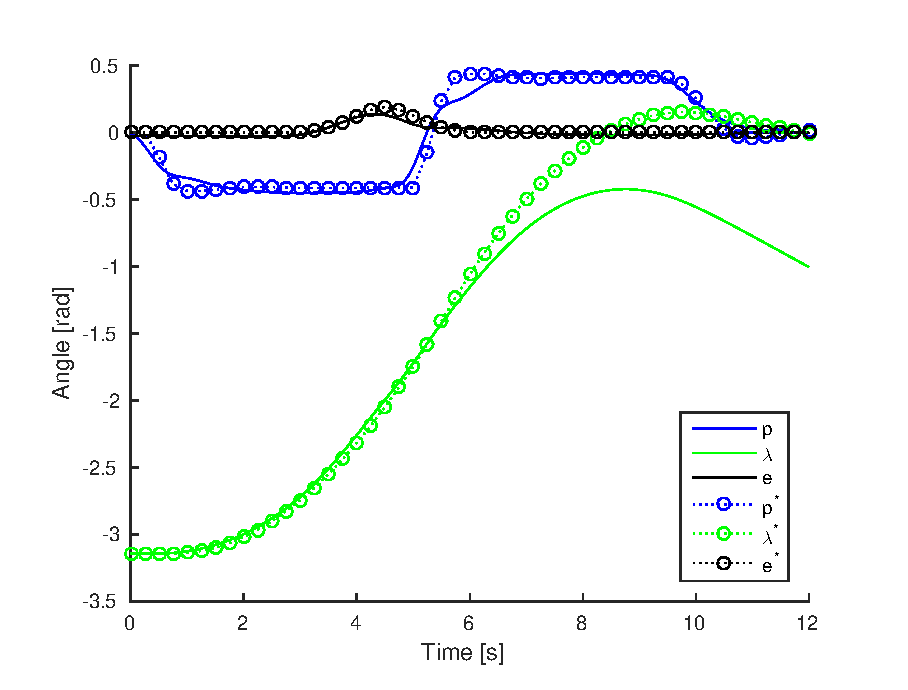
\includegraphics[width=0.85\textwidth]{figures/4/openloop25.eps}
	\caption{Open Loop 25.}
	\label{fig:openloop25}
\end{figure}
\begin{figure}[hp]
	\centering
		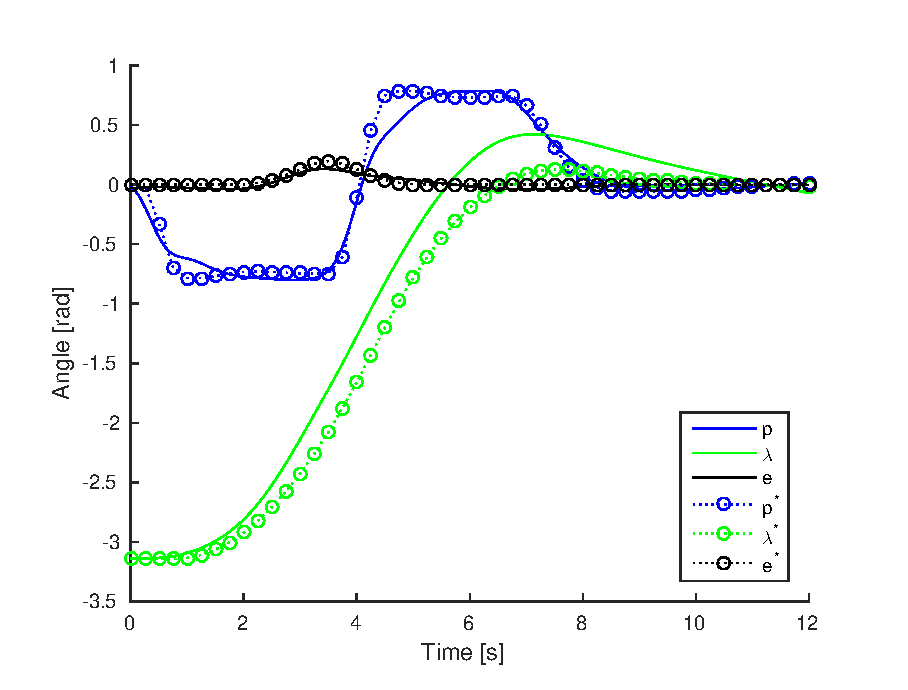
\includegraphics[width=0.85\textwidth]{figures/4/openloop45.eps}
	\caption{Open Loop 45.}
	\label{fig:openloop45}
\end{figure}
\begin{figure}[hp]
	\centering
		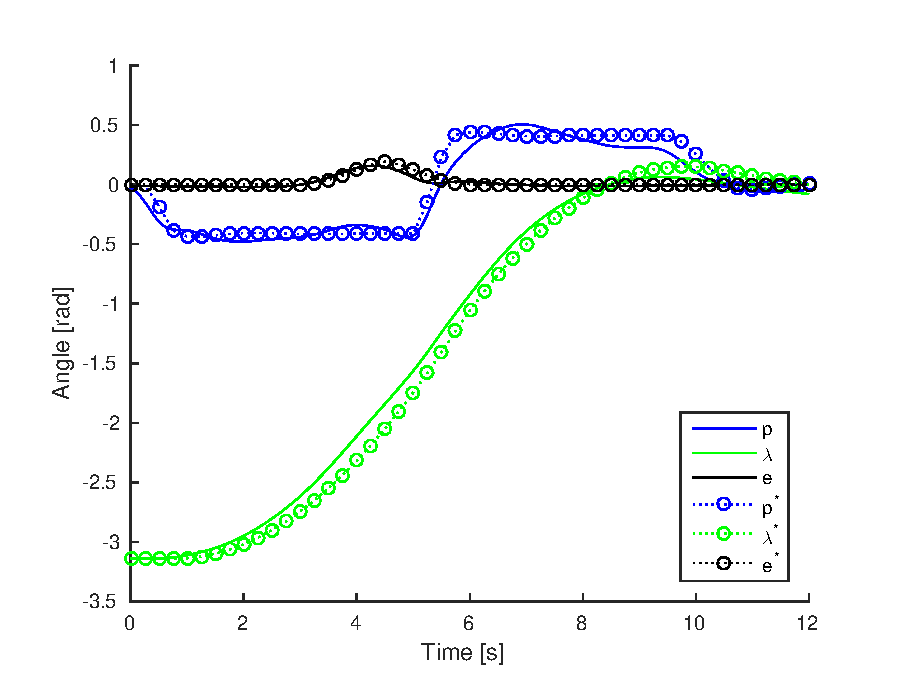
\includegraphics[width=0.85\textwidth]{figures/4/closedloop25.eps}
	\caption{Closed Loop 25.}
	\label{fig:closedloop25}
\end{figure}
\begin{figure}[hp]
	\centering
		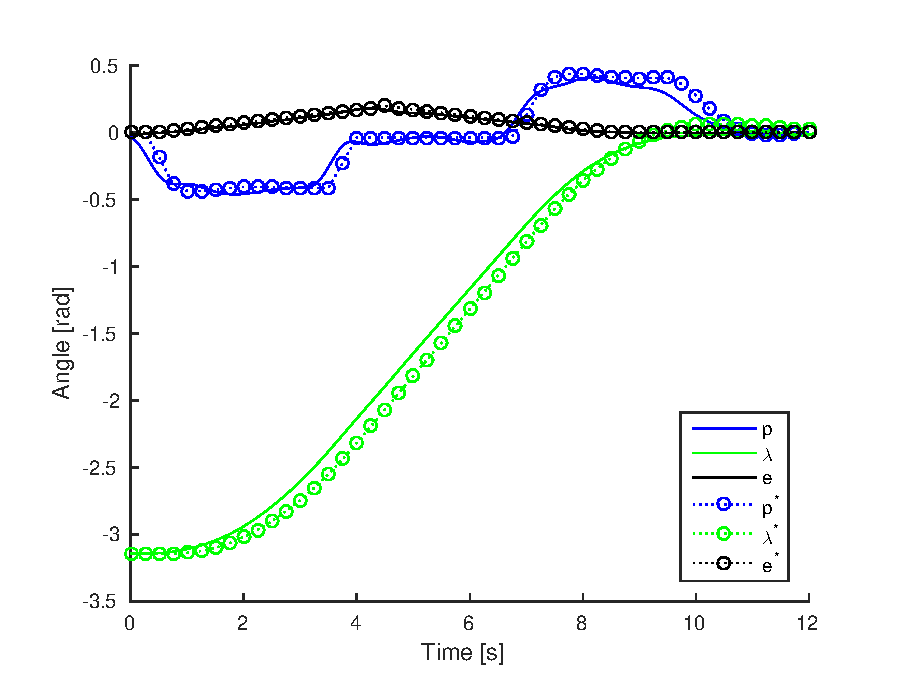
\includegraphics[width=0.85\textwidth]{figures/4/closedloopConstrained25.eps}
	\caption{Closed Loop 25, extra constraints.}
	\label{fig:closedloopConstrained25}
\end{figure}
\begin{figure}[hp]
	\centering
		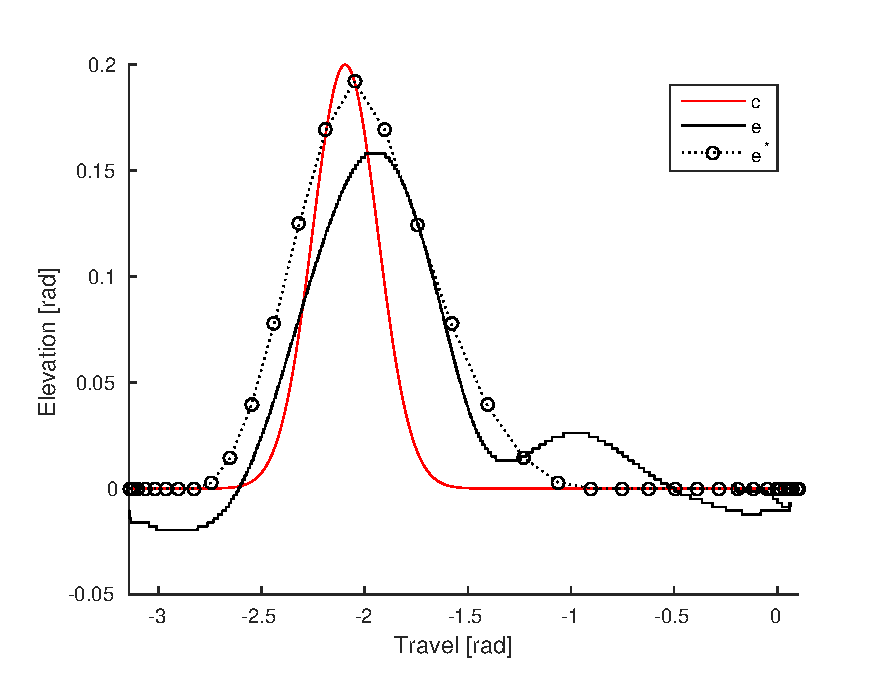
\includegraphics[width=0.85\textwidth]{figures/4/closedloop25_cons.eps}
	\caption{Closed Loop 25 - contraint hill.}
	\label{fig:closedloop25_cons}
\end{figure}
\begin{figure}[hp]
	\centering
		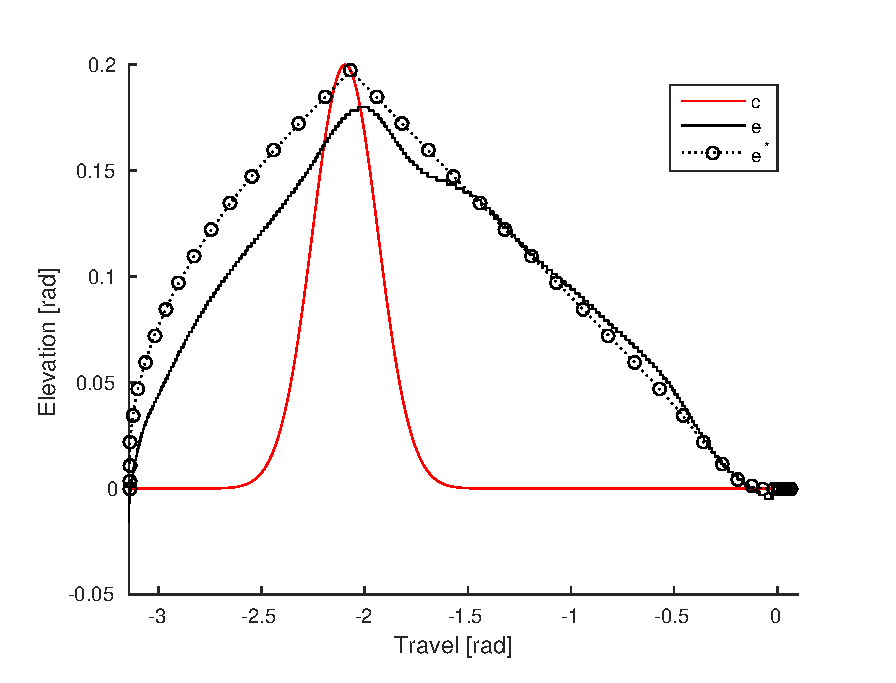
\includegraphics[width=0.85\textwidth]{figures/4/closedloopConstrained25_cons.eps}
	\caption{Closed Loop 25, extra constraints - contraint hill.}
	\label{fig:closedloopConstrained25_cons}
\end{figure}

